\documentclass[letter, 10pt]{article}
\usepackage[utf8]{inputenc}
\usepackage[T1]{fontenc}
\usepackage[spanish]{babel}
\usepackage{amsfonts}
\usepackage{amsmath}
\usepackage{graphicx}
\usepackage{url}
\usepackage[top=3cm,bottom=3cm,left=3.5cm,right=3.5cm,footskip=1.5cm,headheight=1.5cm,headsep=.5cm,textheight=3cm]{geometry}



\begin{document}
\title{Inteligencia Artificial \\ \begin{Large}Estado del Arte: ELECTRIC VEHICLE CHARGING STATION PLACEMENT PROBLEM\end{Large}}
\author{Matias Lara Plaza}
\date{\today}
\maketitle


%--------------------No borrar esta secci\'on--------------------------------%
\section*{Evaluaci\'on}

\begin{tabular}{ll}
Resumen (5\%): & \underline{\hspace{2cm}} \\
Introducci\'on (5\%):  & \underline{\hspace{2cm}} \\
Definici\'on del Problema (10\%):  & \underline{\hspace{2cm}} \\
Estado del Arte (40\%):  & \underline{\hspace{2cm}} \\
Modelo Matem\'atico (20\%): &  \underline{\hspace{2cm}}\\
Conclusiones (15\%): &  \underline{\hspace{2cm}}\\
Bibliograf\'ia (5\%): & \underline{\hspace{2cm}}\\
 &  \\
\textbf{Nota Final (100\%)}:   & \underline{\hspace{2cm}}
\end{tabular}
%---------------------------------------------------------------------------%
\vspace{2cm}


\begin{abstract}
El presente informe aborda el Problema de Ubicación de Estaciones de Carga para 
Vehículos Eléctricos (EVCSPP), un problema de optimización combinatoria NP-duro 
que busca determinar las ubicaciones óptimas para construir estaciones de carga en 
una red urbana, minimizando costos y garantizando que los vehículos puedan 
desplazarse por toda la ciudad sin agotar su autonomía. Se revisan las principales 
aproximaciones propuestas en la literatura, desde métodos exactos hasta algoritmos 
metaheurísticos y técnicas de inspiración cuántica, y se presenta el modelo matemático 
que formaliza el problema. Los hallazgos evidencian que ninguna técnica garantiza el 
óptimo global a gran escala y que la brecha entre modelos teóricos y condiciones 
reales persiste, situando al EVCSPP como un problema abierto con amplias 
oportunidades de investigación futura.
\end{abstract}
\newpage

\section{Introducci\'on}
La dependencia global de los combustibles fósiles ha sido durante décadas uno de los 
principales motores del desarrollo económico y social, pero también una de las fuentes 
más significativas de emisiones de gases de efecto invernadero. El sector del transporte 
es uno de los mayores contribuyentes a esta problemática, siendo responsable de una 
fracción considerable de las emisiones globales de dióxido de carbono. Frente a este 
escenario, la electrificación del transporte ha emergido como una de las respuestas más 
concretas y escalables para reducir la huella ambiental de la movilidad urbana.

En este contexto, diversas regiones del mundo han comenzado a implementar marcos 
regulatorios y políticas públicas orientadas a acelerar la adopción masiva de vehículos 
eléctricos. La Unión Europea, por ejemplo, ha establecido objetivos vinculantes para la 
reducción de emisiones del sector transporte, impulsando tanto la electrificación de la 
flota vehicular como el desarrollo de infraestructura de carga a escala continental. Estas 
iniciativas han generado un crecimiento sostenido en el número de vehículos eléctricos 
en circulación, lo que a su vez ha puesto en evidencia una necesidad crítica: la 
planificación estratégica de las estaciones de carga.

La ubicación de estas estaciones no es un problema trivial. Una red de carga mal 
distribuida puede generar zonas sin cobertura, saturar ciertas ubicaciones y dejar a los 
conductores expuestos a la llamada ansiedad de rango, es decir, el temor a quedarse sin 
energía antes de alcanzar un punto de recarga. Por el contrario, una red bien planificada 
puede extender el alcance efectivo de los vehículos eléctricos a toda el área urbana, 
reducir costos de infraestructura y fomentar la adopción del transporte eléctrico.

El presente informe aborda precisamente este desafío a través del Problema de Ubicación 
de Estaciones de Carga para Vehículos Eléctricos (EVCSPP, por sus siglas en inglés). 
El documento se estructura de la siguiente manera: en primer lugar, se presenta una 
definición formal del problema y sus variantes; a continuación, se desarrolla un estado 
del arte que revisa las principales técnicas propuestas en la literatura para resolverlo; 
posteriormente, se expone el modelo matemático que formaliza el problema de 
optimización; y finalmente, se presentan conclusiones que sintetizan los hallazgos 
y proponen direcciones de investigación futura.

\section{Definici\'on del Problema}

El Problema de Ubicac\'ion de Estaciones de Carga para Veh\'iculos El\'ectricos (EVCSPP, por sus siglas en ingl\'es) surge en el contexto de la electrificaci\'on del transporte, un pilar fundamental para el desarrollo de ciudades inteligentes y la mitigaci\'on de las emisiones de gases de efecto invernadero. A diferencia de las estaciones de combustible tradicionales, la recarga de veh\'iculos el\'ectricos requiere tiempos m\'as prolongados y est\'a limitada por la autonom\'ia de las bater\'ias, lo que genera ansiedad en los conductores. En este escenario, el EVCSPP consiste en determinar las localizaciones geogr\'aficas estrat\'egicas para instalar infraestructuras de carga dentro de una red de transporte, garantizando que los usuarios puedan desplazarse por toda la \'area urbana sin agotar su energ\'ia.

\textbf{El objetivo principal de este problema de optimizaci\'on es minimizar los costos totales del sistema.} Esto abarca fundamentalmente el costo de construcci\'on e instalaci\'on de las estaciones (terrenos, equipos, mantenimiento) y, dependiendo del enfoque, el costo de acceso o transporte, que representa la distancia que los usuarios deben recorrer para llegar a un punto de carga. Este objetivo persigue un equilibrio econ\'omico sin sacrificar la conveniencia de los conductores ni la cobertura del servicio.


La principal dificultad del EVCSPP radica en su elevada complejidad computacional, estando clasificado formalmente como un problema NP-duro \cite{1_Solving_optimal_evcsp_problem_QUANTUM}\cite{2_EVCSP_2013-ieee-conference}.
A medida que aumenta el tama\~no de la red y el n\'umero de ubicaciones candidatas, el espacio de soluciones crece de manera exponencial. La intrincada interdependencia entre m\'ultiples dimensiones (como la infraestructura vial, las limitaciones el\'ectricas y el comportamiento del usuario) hace que los m\'etodos de optimizaci\'on exactos sean ineficientes a gran escala, requiriendo el uso de algoritmos heur\'isticos, metaheur\'isticos o computaci\'on de inspiraci\'on cu\'antica para encontrar soluciones viables.

En la formulaci\'on del problema interact\'uan diversas constantes y variables clave. Las constantes reflejan el entorno f\'isico y econ\'omico: los nodos o sitios candidatos en la ciudad, las distancias entre ellos, la autonom\'ia promedio de los veh\'iculos, la demanda de carga local estimada (basada en el flujo de tr\'afico o densidad poblacional), la capacidad m\'axima de suministro por estaci\'on y los costos fijos asociados a cada locaci\'on. Por su parte, las variables definen el comportamiento del modelo; la principal es una variable de decisi\'on de naturaleza binaria que simplemente indica si se construye o no una estaci\'on en un sitio espec\'ifico\cite{1_Solving_optimal_evcsp_problem_QUANTUM}.

Para que una soluci\'on sea v\'alida, debe cumplir con restricciones operativas y geom\'etricas estrictas. La primera es la restricci\'on de cobertura o alcance, la cual exige que la distancia entre cualquier par de estaciones contiguas no supere la capacidad de conducci\'on aut\'onoma del veh\'iculo, asegurando as\'i una red interconectada. La segunda es la satisfacci\'on de la demanda, que obliga a que la suma de las capacidades de las estaciones operativas en un radio determinado logre cubrir \'integramente las necesidades de carga de los residentes locales\cite{1_Solving_optimal_evcsp_problem_QUANTUM}. Adicionalmente, existen restricciones de asignaci\'on exclusiva que fuerzan a que cada sector de la ciudad est\'e vinculado a una instalaci\'on operativa, y restricciones de equidad territorial para asegurar que la cobertura abarque la totalidad de la zona urbana, incluyendo \'areas remotas o de menor tr\'ansito\cite{1_Solving_optimal_evcsp_problem_QUANTUM}.

Finalmente, a partir de esta estructura cl\'asica, han surgido diversas variantes del problema adaptadas a redes modernas. Destacan los problemas conjuntos de ubicaci\'on y dimensionamiento (sizing), que no solo deciden d\'onde construir sino cu\'anta potencia asignar a cada estaci\'on\cite{2_EVCSP_2013-ieee-conference}; el EVCSPP integrado con sistemas de Veh\'iculo a Red (V2G), donde el autom\'ovil no solo consume sino que provee energ\'ia a la red el\'ectrica\cite{2_EVCSP_2013-ieee-conference}; modelos de planificaci\'on de dos etapas que incorporan la incertidumbre de los Recursos Energ\'eticos Distribuidos (DER), como la energ\'ia solar o e\'olica\cite{3_optimal_placement-metaheuristic}; y las formulaciones basadas en el modelo p-mediano, centradas espec\'ificamente en minimizar la distancia ponderada de viaje de todos los usuarios hacia un n\'umero fijo y predeterminado de estaciones\cite{3_optimal_placement-metaheuristic}.


\section{Estado del Arte}


El estudio de la ubicación espacial de instalaciones tiene sus raíces teóricas a principios del siglo XX con el problema de la planta industrial introducido por Alfred Weber\cite{4_survey_FLP}. Sin embargo, el Problema de Ubicación de Estaciones de Carga para Vehículos Eléctricos (EVCSPP, por sus siglas en inglés) surge en un contexto contemporáneo y diferenciado, impulsado por la imperiosa necesidad de mitigar las emisiones de gases de efecto invernadero procedentes del sector transporte y de reducir la dependencia mundial de los combustibles fósiles\cite{7_recent_trends_optimization_techniques}. Este problema cobra especial relevancia estratégica con la transición hacia el desarrollo de ciudades inteligentes, donde la infraestructura de transporte no solo debe proveer una cobertura espacial sino que también debe integrarse de forma sinérgica y segura con la red eléctrica tradicional\cite{6_EVCSP_formulation_complexity}.

\begin{figure}[h]
    \centering
    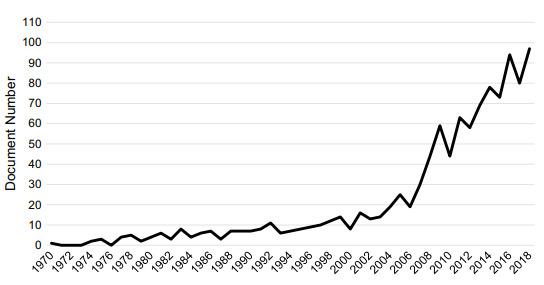
\includegraphics[width=0.7\textwidth]{images/fig1_Celik_Turkoglu.jpg}
    \caption{Evolución anual del número de publicaciones sobre 
    problemas de ubicación de instalaciones de servicio, evidenciando 
    el crecimiento sostenido del campo a partir del año 
    2000 \cite{4_survey_FLP}.}
    \label{fig:publicaciones_anuales}
\end{figure}

\begin{figure}[h]
    \centering
    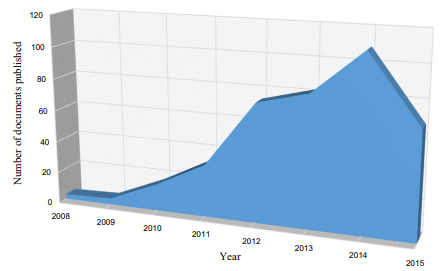
\includegraphics[width=0.7\textwidth]{images/rahman_fig2.png}
    \caption{Número de publicaciones anuales sobre optimización de 
    infraestructura de carga para vehículos eléctricos e híbridos 
    enchufables registradas en bases de datos científicas entre 2008 
    y 2015, reflejando el rápido crecimiento del área de 
    investigación \cite{7_recent_trends_optimization_techniques}.}
    \label{fig:publicaciones_rahman}
\end{figure}


Para abordar este problema, formalmente clasificado por la complejidad computacional como NP-duro, la comunidad científica ha empleado una evolución de enfoques que parten de modelos matemáticos estrictos hacia técnicas de inteligencia artificial. Inicialmente, se aplicaron métodos de optimización exacta, como la programación lineal entero-mixta (MILP) y algoritmos de branch-and-bound, los cuales buscan la optimalidad matemática calculando todas las interacciones posibles\cite{6_EVCSP_formulation_complexity}. No obstante, el crecimiento exponencial del espacio de búsqueda derivado del tamaño de las redes urbanas modernas hizo que estas técnicas resultaran ineficientes y colapsaran en la práctica. Como respuesta, la resolución ha migrado sostenidamente hacia el uso de algoritmos heurísticos y, de manera predominante, métodos metaheurísticos, que sacrifican la garantía absoluta del óptimo a cambio de aproximaciones de alta calidad en tiempos de cómputo razonables\cite{4_survey_FLP}\cite{5_Metaheuristic_FLP}.

En cuanto a las representaciones que han logrado modelar la complejidad del EVCSPP de forma más efectiva, destacan los algoritmos poblacionales y las rutinas basadas en memoria adaptativa. Históricamente, los Algoritmos Genéticos (GA) y la Búsqueda Tabú (TS) han sido las representaciones discretas dominantes para problemas de ubicación de instalaciones, demostrando gran flexibilidad en redes no capacitadas y modelos de p-mediano\cite{5_Metaheuristic_FLP}. Más recientemente, representaciones basadas en inteligencia de enjambres, como la Optimización por Enjambre de Partículas (PSO) y metaheurísticas inspiradas en la naturaleza, como la Optimización por Reacción Química (CRO), han demostrado ser excepcionalmente eficaces\cite{6_EVCSP_formulation_complexity}\cite{7_recent_trends_optimization_techniques}.La efectividad de estas representaciones radica en su intrínseca capacidad de resistencia frente a la escala del problema, permitiendo explorar vastas regiones del espacio de soluciones y evadir los óptimos locales mediante un equilibrio dinámico entre la diversificación (exploración) y la intensificación (explotación) de las alternativas\cite{6_EVCSP_formulation_complexity}\cite{7_recent_trends_optimization_techniques}.

Los resultados más destacados obtenidos hasta la fecha muestran una clara bifurcación operativa en función de la envergadura del escenario analizado. Para microrredes o instancias con un número reducido de nodos (generalmente por debajo de 150), los solucionadores exactos comerciales logran la optimalidad absoluta, aunque a expensas de un alto costo temporal\cite{6_EVCSP_formulation_complexity}. Por el contrario, en problemas a escala urbana, las técnicas metaheurísticas ostentan los resultados más sólidos: mientras que representaciones como GA han dominado consistentemente en tiempos de resolución computacional frente a otros métodos en problemas de cobertura máxima, algoritmos avanzados como CRO han probado superar ampliamente a los métodos constructivos o codiciosos (greedy), logrando convergencias ultra-rápidas hacia el óptimo global sin padecer los déficits de memoria que inutilizan a los modelos puramente matemáticos\cite{5_Metaheuristic_FLP}\cite{6_EVCSP_formulation_complexity}.

\begin{figure}[h]
    \centering
    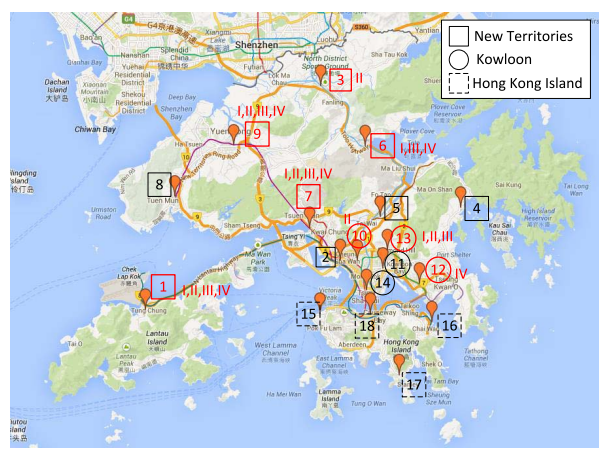
\includegraphics[width=0.6\textwidth]{images/lam_fig4.png}
    \caption{Distribución geográfica de ubicaciones seleccionadas para 
    la construcción de estaciones de carga en Hong Kong, correspondiente 
    a una aplicación real del EVCSPP resuelta mediante métodos exactos 
    y metaheurísticos \cite{6_EVCSP_formulation_complexity}.}
    \label{fig:mapa_hk}
\end{figure}

La tendencia actual de la investigación se está alejando progresivamente de la optimización simple y de las metaheurísticas puras para adentrarse en el desarrollo de técnicas híbridas y algoritmos de optimización multiobjetivo\cite{5_Metaheuristic_FLP}\cite{7_recent_trends_optimization_techniques}.
Las limitaciones de los métodos tempranos, que evaluaban únicamente el costo de instalación de las estaciones o la cobertura espacial del usuario, han propiciado el diseño de modelos complejos (como NSGA-II o MOPSO) que equilibran de manera simultánea factores en conflicto, como el costo de la red, el 'afeitado de picos' de la demanda eléctrica y el desgaste de las baterías\cite{7_recent_trends_optimization_techniques}. Hacia el futuro, el estado del arte se dirige invariablemente a integrar el despliegue físico de las estaciones con sistemas de Gestión de la Demanda (DSM), la implementación de arquitecturas de Vehículo a Red (V2G) y el acoplamiento directo de fuentes de energía renovable, particularmente la tecnología fotovoltaica, con el propósito de descentralizar la carga y proteger la integridad operativa de la red eléctrica principal\cite{7_recent_trends_optimization_techniques}.


\section{Modelo Matem\'atico}

El presente modelo matemático se basa en la formulación propuesta por Ou et al. (2025) \cite{1_Solving_optimal_evcsp_problem_QUANTUM}, 
quienes extienden el trabajo seminal de Lam et al. (2013) \cite{2_EVCSP_2013-ieee-conference} incorporando restricciones 
adicionales de cobertura urbana y zonas remotas. El problema consiste en determinar las 
ubicaciones óptimas para la construcción de estaciones de carga de vehículos eléctricos, 
minimizando el costo total de construcción y garantizando que la red resultante satisfaga 
criterios de accesibilidad, demanda y cobertura territorial.

\subsection{Conjuntos y Parámetros}

Se define un grafo no dirigido $G = (V, E)$, donde $V$ representa el conjunto de ubicaciones 
candidatas para la construcción de estaciones de carga y $E$ el conjunto de aristas que conectan 
dichas ubicaciones. A partir de un coeficiente de descuento $\alpha \in [0, 1)$ y el rango de 
autonomía promedio $R$, se define el subconjunto de nodos relevantes como:

\[
\bar{V} = \{j \in V \mid \alpha R \leq d(i,j) \leq R,\ i \neq j\}
\]

donde $d(i,j)$ denota la distancia entre los nodos $i$ y $j$. Este conjunto captura las 
ubicaciones que se encuentran suficientemente alejadas entre sí para evitar concentración 
excesiva de estaciones, pero dentro del rango de autonomía del vehículo.

Los parámetros del modelo se describen en el Cuadro~\ref{tab:parametros}.

\begin{table}[h]
\centering
\caption{Parámetros del modelo matemático}
\label{tab:parametros}
\begin{tabular}{cl}
\hline
\textbf{Parámetro} & \textbf{Descripción} \\
\hline
$C_j$       & Costo de construcción de la estación en la ubicación $j$, \\
            & incluyendo adquisición de terreno, construcción y operación \\
$R$         & Distancia de autonomía promedio de los vehículos eléctricos \\
$\alpha$    & Coeficiente de descuento que regula la densidad mínima entre estaciones \\
$d(i,j)$   & Distancia entre las ubicaciones $i$ y $j$ \\
$s_j$       & Radio de servicio de la estación en la ubicación $j$ \\
$D_j$       & Demanda de carga en la ubicación $j$ \\
$f_i$       & Capacidad de carga promedio en la ubicación $i$ \\
$\mathit{CityArea}$ & Área total de la ciudad que debe ser cubierta por las estaciones \\
$T$         & Subconjunto de ubicaciones candidatas en zonas remotas \\
\hline
\end{tabular}
\end{table}

\subsection{Variable de Decisión}

La variable de decisión del modelo es binaria e indica si se construye o no una estación 
de carga en cada ubicación candidata:

\[
x_j = \begin{cases} 1 & \text{si se construye una estación en la ubicación } j \\ 
0 & \text{en caso contrario} \end{cases} \quad \forall j \in V
\]

\subsection{Función Objetivo}

Se minimiza el costo total de construcción de las estaciones seleccionadas:

\[
\min \sum_{j=1}^{n} C_j x_j \quad \forall j \in V \tag{1}
\]

La función objetivo busca determinar el subconjunto de ubicaciones candidatas sobre las 
cuales construir estaciones de carga, de manera que la suma de los costos de construcción 
de las estaciones seleccionadas sea mínima, sujeto a que se satisfagan las restricciones 
de accesibilidad, demanda, cobertura y zonas remotas definidas a continuación.

\subsection{Restricciones}

\textbf{Restricción de accesibilidad:} Se garantiza que desde cualquier estación construida 
sea posible alcanzar al menos otra estación dentro del rango de autonomía del vehículo 
eléctrico. Es decir, para cada arista $(i,j)$ perteneciente al grafo $\bar{G} = (\bar{V}, \bar{E})$, 
al menos uno de sus extremos debe tener una estación construida:

\[
x_i + x_j \geq 1 \quad \forall (i,j) \in \bar{E} \tag{2}
\]

Esta restricción asegura la continuidad de la red de carga, de modo que ningún vehículo 
quede varado al agotar su autonomía.

\textbf{Restricción de satisfacción de demanda:} La capacidad de carga total aportada por 
las estaciones construidas en el entorno de cada nodo $j$ debe ser suficiente para cubrir 
la demanda local de carga:

\[
\sum_{i \in \bar{V}_j^{\alpha R}} f_i x_i \geq D_j \quad \forall j \in V \tag{3}
\]

donde $\bar{V}_j^{\alpha R}$ denota el conjunto de estaciones ubicadas a una distancia 
entre $\alpha R$ y $R$ del nodo $j$. Esta restricción garantiza que cada zona de la ciudad 
cuente con suficiente infraestructura de carga para atender a los vehículos eléctricos 
de su área.

\textbf{Restricción de cobertura urbana:} La suma de los radios de servicio de todas las 
estaciones construidas debe ser al menos igual al área total de la ciudad:

\[
\sum_{j=1}^{n} s_j x_j \geq \mathit{CityArea} \quad \forall j \in V \tag{4}
\]

Esta restricción asegura que el conjunto de estaciones seleccionadas provea cobertura 
geográfica sobre la totalidad del territorio urbano considerado.

\textbf{Restricción de zonas remotas:} Se exige que al menos una estación de carga sea 
construida en alguna de las ubicaciones identificadas como remotas o periféricas, con el 
fin de garantizar la accesibilidad en sectores de menor densidad de vehículos eléctricos:

\[
\sum_{j \in T} x_j \geq 1 \tag{5}
\]

Esta restricción responde a criterios de equidad territorial, evitando que la optimización 
de costos derive en una concentración exclusiva de estaciones en zonas de alta densidad 
urbana.


\section{Conclusiones}

El análisis comparativo de las técnicas estudiadas para resolver el Problema de Ubicación 
de Estaciones de Carga para Vehículos Eléctricos (EVCSPP) permite extraer conclusiones 
relevantes tanto sobre el estado actual de la investigación como los problemas que 
permanecen activos y constituyen oportunidades concretas de avance.

En primer lugar, se constata que las técnicas revisadas no resuelven exactamente el mismo 
problema. Si bien todas comparten el objetivo central de minimizar costos de construcción 
sujeto a restricciones de cobertura y accesibilidad, existen diferencias sustanciales en su 
formulación. El trabajo de Lam et al.(2013 y 2014) \cite{2_EVCSP_2013-ieee-conference, 6_EVCSP_formulation_complexity} se centra en garantizar la 
conectividad topológica de la red mediante un modelo de flujo en grafos. Ou et al. 
\cite{1_Solving_optimal_evcsp_problem_QUANTUM} extiende esta formulación incorporando restricciones de cobertura del área 
urbana total y equidad territorial. Por su parte, Demiryürek et al. \cite{3_optimal_placement-metaheuristic} 
adopta una perspectiva distinta a través del modelo p-mediano, donde el foco recae en 
minimizar la distancia ponderada de acceso de los usuarios, prescindiendo del requisito 
explícito de conectividad entre estaciones. Esta diversidad de formulaciones refleja que 
el EVCSPP no es un problema resuelto ni consensuado: cada enfoque modela una versión 
distinta de la realidad, y ninguno captura la totalidad de sus dimensiones de manera 
simultánea.

En lo que respecta a las similitudes, todas las técnicas revisadas coinciden en representar 
el problema mediante variables de decisión binarias, en reconocer su complejidad 
computacional NP-dura y en recurrir a métodos que, en mayor o menor medida, sacrifican 
la garantía de optimalidad a cambio de eficiencia computacional. Esta última característica 
constituye precisamente la limitación más crítica y transversal identificada en la revisión: 
ninguna de las técnicas estudiadas puede garantizar la obtención del óptimo global a gran 
escala. Los métodos exactos basados en programación lineal entero-mixta (MILP) colapsan 
ante instancias urbanas reales por restricciones de memoria. Las metaheurísticas como los 
algoritmos genéticos (GA) y la optimización por colonia de hormigas (ACO) ofrecen 
soluciones de buena calidad, pero sin certeza de optimalidad y con sensibilidad a la 
configuración de parámetros. Incluso el recocido cuántico digital (DA3), la técnica más 
avanzada de las revisadas, entrega soluciones de alta calidad en tiempos competitivos, 
pero opera bajo el paradigma de inspiración cuántica y no bajo computación cuántica real.
Esto significa que, a diferencia de un computador cuántico genuino como los aniladores 
D-Wave, el DA3 ejecuta sus cálculos en hardware clásico simulando el comportamiento del 
túnel cuántico mediante reglas probabilísticas. Por lo tanto, aunque en la práctica 
demuestra tiempos de cómputo más rápidos y soluciones de menor costo que GA y SA, 
no existe una demostración teórica de que explore el espacio de soluciones de manera 
fundamentalmente distinta a otras metaheurísticas avanzadas. En otras palabras, el DA3 
puede quedar atrapado en óptimos locales exactamente de la misma forma que cualquier 
otro algoritmo de búsqueda estocástica, y la garantía de encontrar el óptimo global 
sigue siendo una cuestión abierta tanto para él como para el resto de las técnicas revisadas.

En consecuencia, el EVCSPP permanece como un problema abierto. La comunidad científica 
ha avanzado considerablemente en la eficiencia computacional y en la riqueza de las 
formulaciones, pero la brecha entre los modelos teóricos y las condiciones operacionales 
reales sigue siendo amplia. \textbf{Los modelos actuales asumen parámetros estáticos: costos fijos, demandas constantes y rangos de autonomía uniformes, cuando en la práctica estos valores varían según la hora del día, las condiciones climáticas, el estado de carga de cada vehículo y los patrones de movilidad de la población.}

Por lo anteriormente expuesto, resulta evidente que una dirección prioritaria para la 
investigación futura consiste en someter los modelos existentes, en particular el de 
recocido cuántico digital, a validaciones con datos reales y de mayor complejidad. 
Los estudios revisados trabajan con parámetros generados aleatoriamente o estimados 
a partir de supuestos simplificadores, lo que limita la capacidad de evaluar su 
desempeño en condiciones operacionales genuinas. Sería de gran valor que trabajos 
futuros incorporen series temporales de flujo de tráfico, registros históricos de 
carga de vehículos eléctricos, variaciones estacionales de la demanda energética y 
datos de movilidad urbana obtenidos de fuentes abiertas. Esta integración permitiría 
transformar los modelos actuales desde ejercicios de optimización sobre parámetros 
supuestos hacia herramientas de planificación operacional capaces de adaptarse a la 
incertidumbre real del comportamiento de los usuarios y de los sistemas de transporte.



\newpage

\section{Uso LLMs}

\begin{enumerate}
    \item Herramienta: Gemini 3.1 flash (Versión promocional estudiantes)
    \item Uso: Revisión de redacción, Resumen de fuentes, Depurar errores de latex.
    \item Prompt principal: Consultas información específica en fuentes: "De acuerdo a este \{abstract\} y a esta \{conclusión\} del recurso \{recurso\} se habla de \{tema\}?"
    \item Intervención: Si la IA me confirmaba o me negaba preguntas que tenía sobre una fuente, iba de nuevo a revisar la parte del texto con la que estaba (o no estaba) siendo coherente con mi idea.
\end{enumerate}

\bibliographystyle{plain}
\bibliography{Referencias}

\end{document} 
